\chapter{Discussion of Results}

\section{Experiment Configuration}
For this experiment 10 random worlds were generated each with 2 mobile targets, 4 static targets, and 5 UAVs.  The simulated worlds were configured as a 2.5 by 2.5$km$ area subdivided into 15 rows and columns.  A rendering of each generated world is included in section~\ref{sec:world_images}.

The mobile targets moved at $10m/s$ and were best hit from $\pm115^{\circ}$ from their front.  Static targets were best hit from $\pm45^{\circ}$.

Two types of UAVs were modeled.  One is a fast long range ISR platform and the other is a slow strike platform.  The ISR platform is type 0 in table~\ref{tab:uavKinematic}.  The strike platform is type 1 in table~\ref{tab:uavKinematic}.  The ISR platform carries sensor 0 defined in table~\ref{tab:sensorType} and has no weapons.  The strike platform has sensor type 1 defined in table~\ref{tab:sensorType}.  The strike platform carries 4 rounds each of weapon types 0 and 1 defined in table~\ref{tab:weaponType}.  Ideally this is more than enough munitions to complete the missions even with a significant amount of misses.  The performance of these sensors and weapons against the targets are defined in tables~\ref{tab:snsrTgtProb}, ~\ref{tab:snsrTgtMisClassProb}, and \ref{tab:wpnTgtProb}.  Static targets are target type 0 and mobile targets are type 1.  The sensors all have a $10\%$ chance of misclassifying any target type as the other type as listed in ~\ref{tab:snsrTgtMisClassProb}.

The simulation was ran for all 10 worlds with the same random seed.  This process was repeated 5 times in order to measure the effects on mission performance with a varying communication range.  The results of these simulation runs were averaged together and are shown in table~\ref{tab:avgResults} and plotted in figure~\ref{fig:averages}.  The complete raw time data per world and per communication range can be found in section~\ref{sec:raw_data}.

\begin{table}[H]
	\caption{Average time to complete objectives}
	\centering
	\rowcolors{1}{lightgray}{white}
	\label{tab:avgResults}
	\begin{tabular}{|p{1.25cm}|p{1.5cm}|p{1.75cm}|p{1.5cm}|}
		\hline
		Comm. Range \% & Average time all detected (s) & Average time all destroyed (s) & Average time world known (s)\\
		\hline
		100 & 116 & 206 & 61  \\ \hline
		20  & 151 & 239 & 90  \\ \hline
		10  & 116 & 231 & 95  \\ \hline
		5   & 238 & 279 & 242 \\ \hline
		2   & 380 & 554 & 339 \\ \hline
	\end{tabular}
\end{table}

\section{General Results}

The $100\%$ communication range case serves as a comparative baseline against a perfect global communication network.  In this case all UAVs are able to communicate with all other UAVs at all times.  As expected a perfect global and centralized communication network always performs better than a network with limited ranges.  The interesting point of comparison is that the $10\%$ and $20\%$ range cases come very close or match the $100\%$ case in performance.  This can be seen in figure~\ref{fig:averages} and in the ratios listed in table~\ref{tab:avgResultsRatio}.

\begin{table}[H]
	\caption{Ratio of time to complete objectives compared to 100\% range}
	\centering
	\rowcolors{1}{lightgray}{white}
	\label{tab:avgResultsRatio}
	\begin{tabular}{|p{1.25cm}|p{1.5cm}|p{1.75cm}|p{1.5cm}|}
		\hline
		Comm. Range \% & Average time all detected ratio & Average time all destroyed ratio & Average time world known ratio\\
		\hline
		100 & 1.0   & 1.0   & 1.0  \\ \hline
		20  & 1.302 & 1.160 & 1.475  \\ \hline
		10  & 1.0   & 1.121 & 1.557  \\ \hline
		5   & 2.052 & 1.354 & 3.967 \\ \hline
		2   & 3.276 & 2.690 & 5.557 \\ \hline
	\end{tabular}
\end{table}

The similar performances can be attributed to the number of UAVs in the swarm.  This simulation used 5 UAVs.  If each of the 5 UAVs can cover $20\%$ of the world then in affect we've created a global network that is only separated by up a few relay hops.  Similarly the $10\%$ case covers half the world most of the time with 5 UAVs.  Conversely, the $5\%$ and $2\%$ cases can only cover a small fraction of the world at best and therefore their performance is much worse than the baseline $100\%$ case.



The $20\%$ and $10\%$ cases are not as heavily pressured as the shorter range cases to react to targets immediately.  These longer range cases can afford to wait for the most appropriate UAV to become available for the monitor and strike tasks so their average time to Destroy is roughly double that of their time to Detect everything.  The UAVs do not have to focus as much time on search and exploration tasking to maintain world certainty and keep Shannon entropy to a minimum.

\end{multicols*}

\begin{figure}[H]
	\centering
	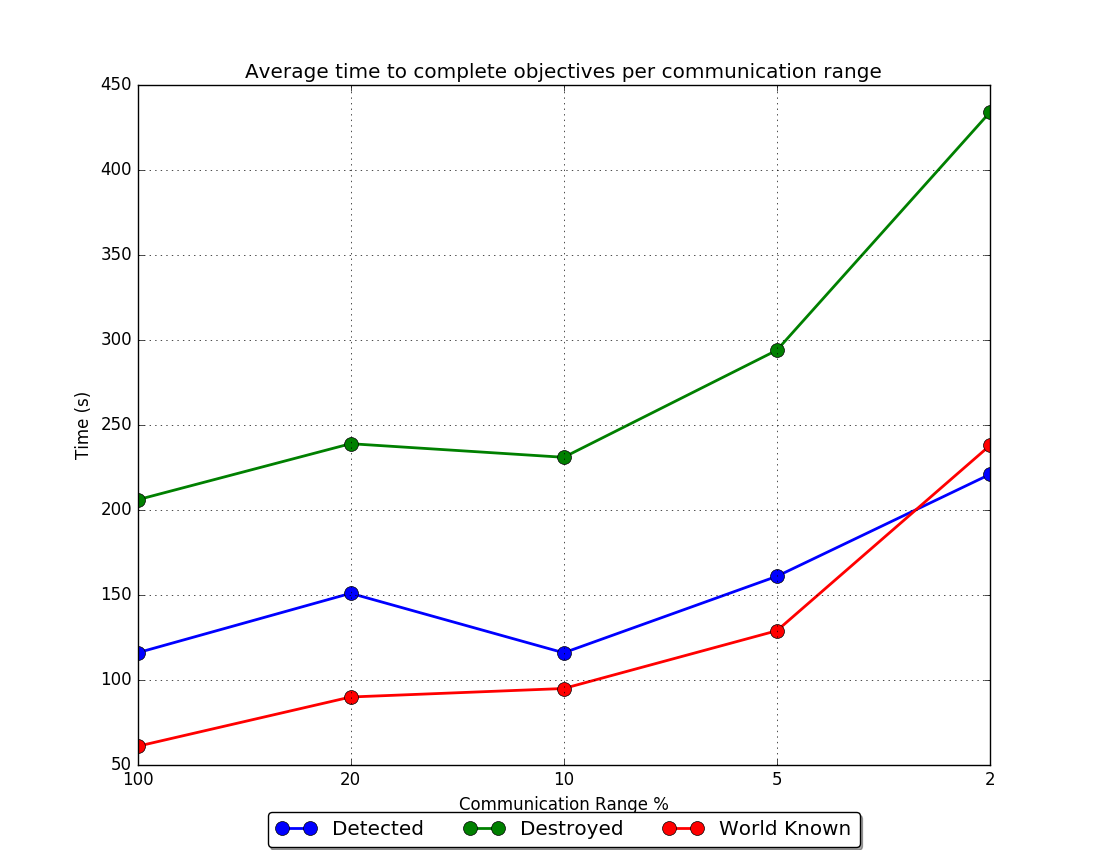
\includegraphics[width=\linewidth,height=4in,keepaspectratio=false]{averages.png}
	\caption{Average time to complete objectives per communication range}
	\label{fig:averages}
\end{figure}

\begin{multicols*}{2}

In contrast, the shorter range cases must react quickly once a target is found otherwise there is a strong possibility it will be lost.  This explains why the average time for Detections and World Known are near equal in the $5\%$ case with the average Destroyed time not far behind.  Once a target is seen it is immediately destroyed.

The $2\%$ case shows a similar trend in the time necessary for Detecting and World Known but the Destroyed time is drastically slower.  This is likely because the much shorter range requires the UAVs to frequently give up Monitoring a target since no strike platform is around before the Monitor time out occurs.  In the $2\%$ case the only time a target is struck is when 2 UAVs happen to be near each other when the target is found or a strike UAV happens to be exploring a part of the world it thinks is highly uncertain.  The strike platform will synchronize with the Monitoring UAV and immediately begin the attack process, assuming it has munitions available, otherwise it will have to relay the message to someone else in the swarm.

Within the performance limits and size of the swarm in these simulations we can see that there is no absolute need for every member of a swarm to be able to reach all others in a global fashion.  In practice with standard RF equipment this is actually undesirable because the UAVs will constantly be jamming each other inadvertently.  The standard trade off is finding a suitable transmission range that allows sufficient bandwidth and world coverage between members of the swarm.  Another real world constraint on RF transmissions is the desire to remain undetected.  By limiting our transmission range and power we can limit the range of detectability by enemy RF sensors.  Within the constraints of this simulation we can drop the transmission range down to $10\%$ of the maximum world range with almost no detrimental affects on overall mission performance.  If some performance degradation is acceptable we can further reduce the communication range requirements to $5\%$.  It seems extreme but is also possible to still complete the mission with only a $2\%$ communication range albeit with a much longer mission duration and risk of failure.

\section{Unique Results}
There are a few results where the swarm was unable to complete the mission.  World 3 was a problem for the $100\%$, $10\%$, and $2\%$ cases.  World 3 can be seen in figure~\ref{fig:world3}.  There is a static target located at row 9 column 0.  The best approach angle for striking a static target is $\pm45^{\circ}$.  In this literal edge case that approach angle puts the UAVs on a trajectory outside of the world.  Therefore the UAVs will attempt strikes at very poor angles from the target's backside instead.  The logs show that many shots are taken at this target and miss.  Eventually all of the strike platforms run out of munitions on this target unless they get very lucky.  This result is a limitation of the simulation's random generation nature.  A real world mission analyst would expand the mission area to allow for a better strike angle against this target.  The simulation does not account for accumulating damage.  Every strike is a boolean draw to decide if a target is destroyed or not.  So even though in the simulation dozens of shots were fired at the target it is still considered alive and well.  In the real world dozens of shots would have likely caused significant if not fatal damage to the target even when fired from an undesirable angle.

Communication range case of $5\%$ failed to complete world 4 and case $2\%$ failed to complete world 9.  In both cases a mobile target survived.  The logs show that the Attack platforms and the Monitoring platforms were not in communication range in both cases.  This compounded into multiple problems and possible failure issues.  The strike UAVs, who are the only armed aircraft, have very poor sensors compared to the ISR platforms.  The Attack platforms have a hard time finding and tracking mobile targets with these poor sensors.  Since the Attack and Monitor aircraft were not in communication range the Attack platforms usually had out-dated information and therefore had a tendency to fire where the mobile target was in the past instead of where it is now.  

Another compounding issue in these short communication range cases is that the Monitoring UAVs were strike platforms instead of ISR platforms.  In these cases a strike platform would happen upon a target but no ISR platforms were able to hear about the target announcement.  Therefore the strike platform would perform the Monitoring task and do a poor job of it.  It would follow the mobile target while requesting for a second strike platform to perform the Attack task.  When a strike platform began performing the Attack it would suffer from the same poor sensor issues as the Monitoring platform, leading to many shots at where a target ``was'' instead of where it really ``is.''


